\documentclass{standalone}
\usepackage{tikz}
\usetikzlibrary{patterns, positioning}
\usepackage[sfdefault]{ClearSans} %% option 'sfdefault' activates Clear Sans as the default text font
\usepackage[T1]{fontenc}

\begin{document}
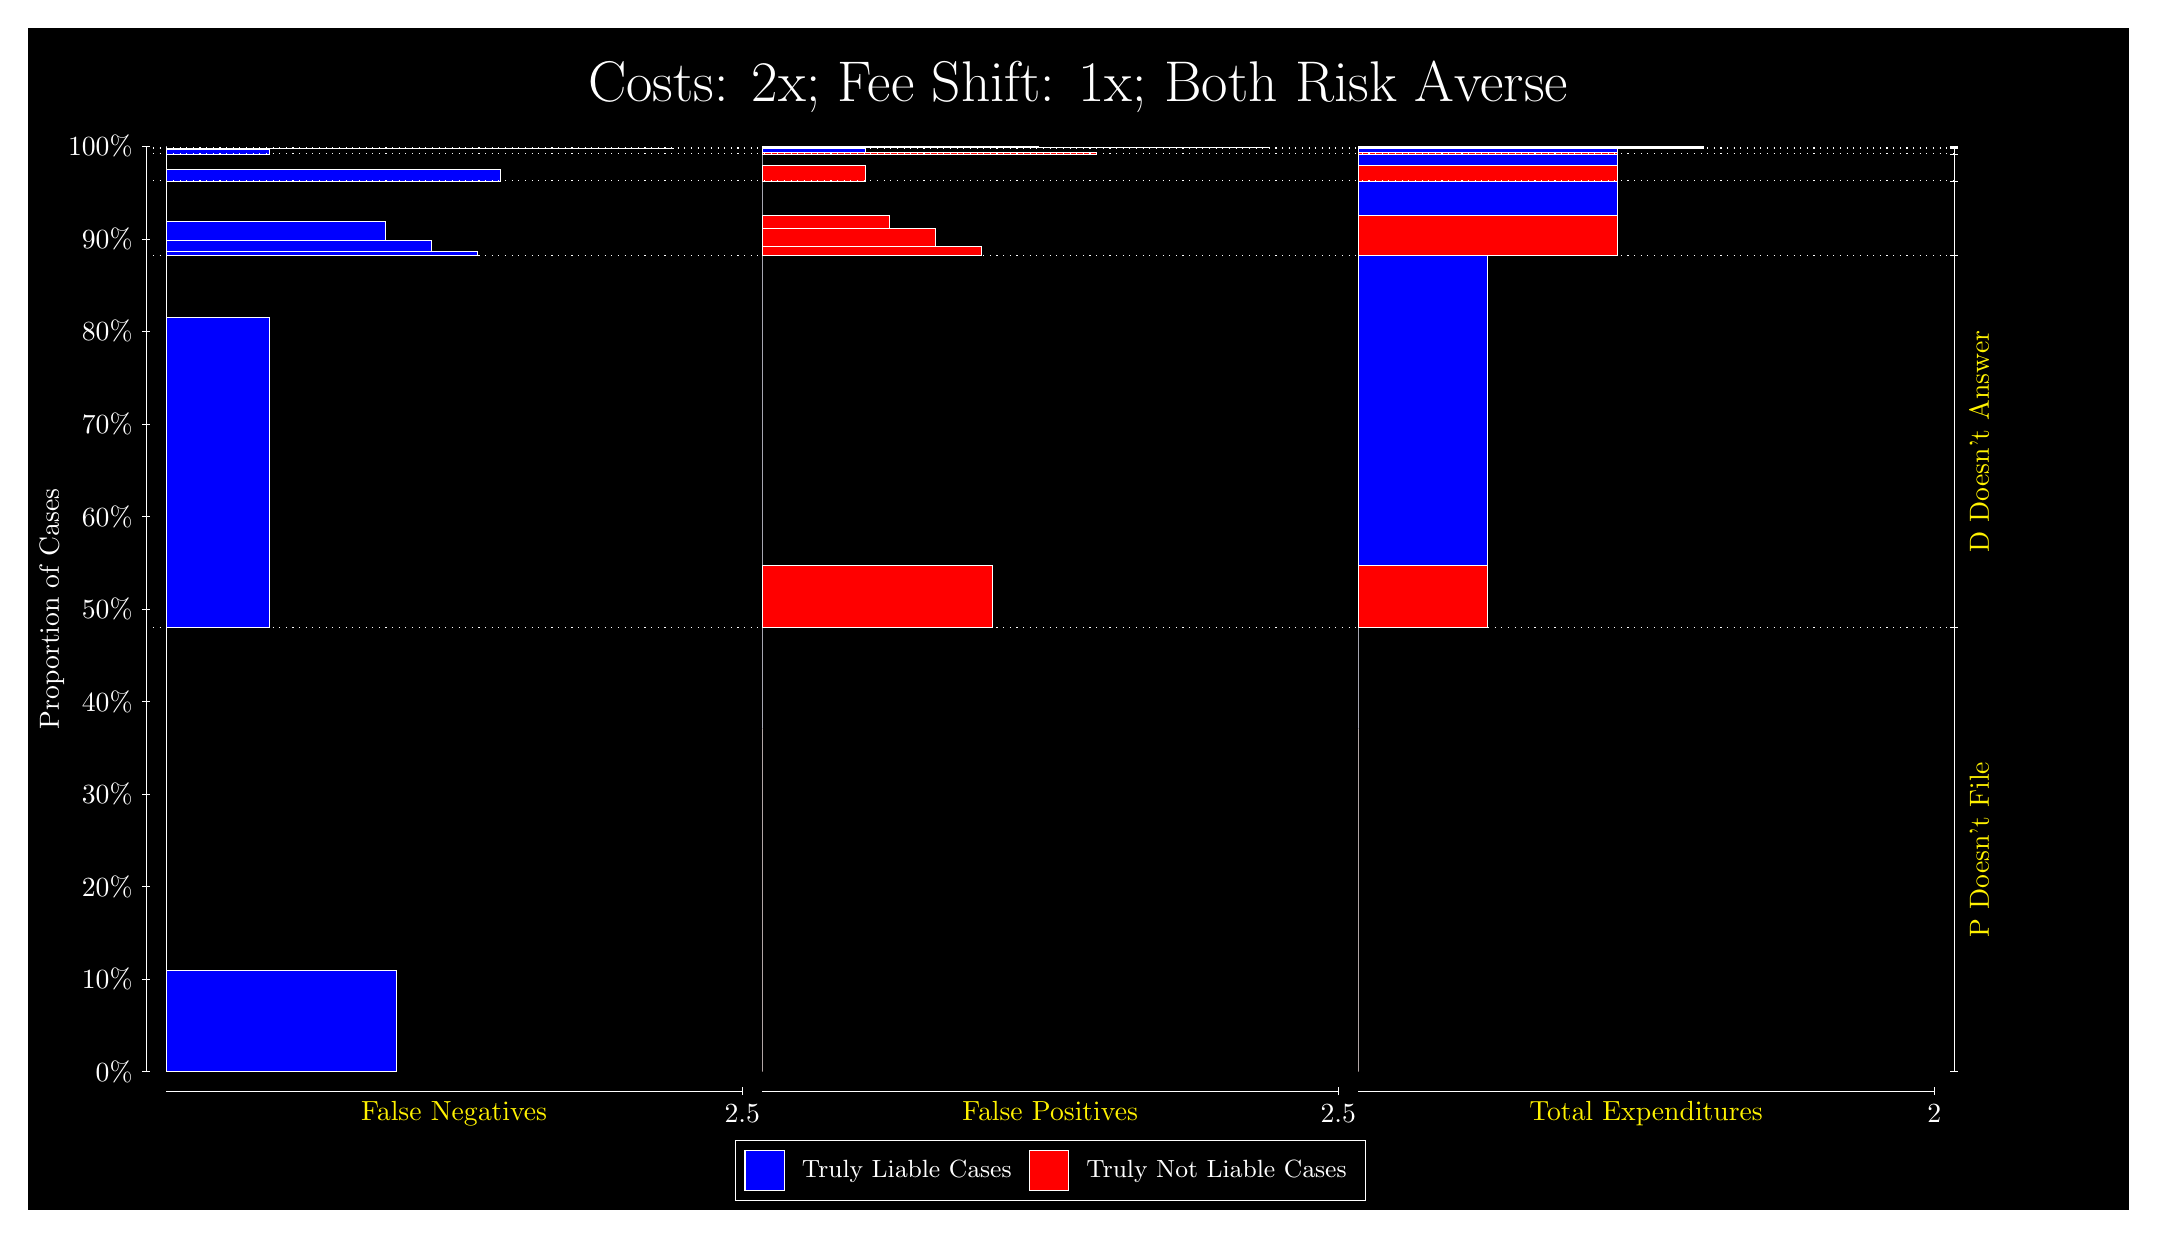
\begin{tikzpicture}
\draw[fill=black] (0,0) rectangle (26.667,15);
\draw[text=white] (0,13.5) rectangle (26.667,15) node[midway] {\huge Costs: 2x; Fee Shift: 1x; Both Risk Averse};
\draw[white, very thin] (1.5,1.75) -- (1.5,13.5);
\node[rotate=90, text=white, anchor=center] at (0.3, 7.625) {Proportion of Cases};
\draw[white, very thin] (1.45,1.75) -- (1.55,1.75);
\node[text=white, anchor=east] at (1.45, 1.75) {0\%};
\draw[white, very thin] (1.45,2.925) -- (1.55,2.925);
\node[text=white, anchor=east] at (1.45, 2.925) {10\%};
\draw[white, very thin] (1.45,4.1) -- (1.55,4.1);
\node[text=white, anchor=east] at (1.45, 4.1) {20\%};
\draw[white, very thin] (1.45,5.275) -- (1.55,5.275);
\node[text=white, anchor=east] at (1.45, 5.275) {30\%};
\draw[white, very thin] (1.45,6.45) -- (1.55,6.45);
\node[text=white, anchor=east] at (1.45, 6.45) {40\%};
\draw[white, very thin] (1.45,7.625) -- (1.55,7.625);
\node[text=white, anchor=east] at (1.45, 7.625) {50\%};
\draw[white, very thin] (1.45,8.8) -- (1.55,8.8);
\node[text=white, anchor=east] at (1.45, 8.8) {60\%};
\draw[white, very thin] (1.45,9.975) -- (1.55,9.975);
\node[text=white, anchor=east] at (1.45, 9.975) {70\%};
\draw[white, very thin] (1.45,11.15) -- (1.55,11.15);
\node[text=white, anchor=east] at (1.45, 11.15) {80\%};
\draw[white, very thin] (1.45,12.325) -- (1.55,12.325);
\node[text=white, anchor=east] at (1.45, 12.325) {90\%};
\draw[white, very thin] (1.45,13.5) -- (1.55,13.5);
\node[text=white, anchor=east] at (1.45, 13.5) {100\%};

\draw[white, very thin] (24.457,1.75) -- (24.457,13.5);
\draw[white, very thin] (24.407,1.75) -- (24.507,1.75);
\node[anchor=west] at (24.407, 1.75) {};
\draw[white, very thin] (24.407,7.3864) -- (24.507,7.3864);
\node[anchor=west] at (24.407, 7.3864) {};
\draw[white, very thin] (24.407,12.111) -- (24.507,12.111);
\node[anchor=west] at (24.407, 12.111) {};
\draw[white, very thin] (24.407,13.061) -- (24.507,13.061);
\node[anchor=west] at (24.407, 13.061) {};
\draw[white, very thin] (24.407,13.404) -- (24.507,13.404);
\node[anchor=west] at (24.407, 13.404) {};
\draw[white, very thin] (24.407,13.475) -- (24.507,13.475);
\node[anchor=west] at (24.407, 13.475) {};
\draw[white, very thin] (24.407,13.484) -- (24.507,13.484);
\node[anchor=west] at (24.407, 13.484) {};
\draw[white, very thin] (24.407,13.5) -- (24.507,13.5);
\node[anchor=west] at (24.407, 13.5) {};

\draw[white, very thin, fill=blue] (1.75,1.75) rectangle (4.6775,3.0331);
\draw[white, very thin, fill=red] (1.75,3.0331) rectangle (1.75,7.3864);
\draw[white, very thin, fill=blue] (1.75,7.3864) rectangle (3.0674,11.324);
\draw[white, very thin, fill=red] (1.75,11.324) rectangle (1.75,12.111);
\draw[white, very thin, fill=blue] (1.75,12.111) rectangle (5.7022,12.164);
\draw[white, very thin, fill=blue] (1.75,12.164) rectangle (5.1167,12.309);
\draw[white, very thin, fill=blue] (1.75,12.309) rectangle (4.5312,12.553);
\draw[white, very thin, fill=red] (1.75,12.553) rectangle (1.75,13.061);
\draw[white, very thin, fill=blue] (1.75,13.061) rectangle (5.9949,13.204);
\draw[white, very thin, fill=red] (1.75,13.204) rectangle (1.75,13.404);
\draw[white, very thin, fill=blue] (1.75,13.404) rectangle (3.0674,13.459);
\draw[white, very thin, fill=red] (1.75,13.459) rectangle (1.75,13.475);
\draw[white, very thin, fill=blue] (1.75,13.475) rectangle (8.1906,13.479);
\draw[white, very thin, fill=red] (1.75,13.479) rectangle (1.75,13.484);
\draw[white, very thin, fill=red] (1.75,13.484) rectangle (1.75,13.488);
\draw[white, very thin, fill=blue] (1.75,13.488) rectangle (1.75,13.5);
\draw[white, very thin, fill=red] (9.3189,1.75) rectangle (9.3189,6.1033);
\draw[white, very thin, fill=blue] (9.3189,6.1033) rectangle (9.3189,7.3864);
\draw[white, very thin, fill=red] (9.3189,7.3864) rectangle (12.246,8.1733);
\draw[white, very thin, fill=blue] (9.3189,8.1733) rectangle (9.3189,12.111);
\draw[white, very thin, fill=red] (9.3189,12.111) rectangle (12.1,12.227);
\draw[white, very thin, fill=red] (9.3189,12.227) rectangle (11.515,12.458);
\draw[white, very thin, fill=red] (9.3189,12.458) rectangle (10.929,12.62);
\draw[white, very thin, fill=blue] (9.3189,12.62) rectangle (9.3189,13.061);
\draw[white, very thin, fill=red] (9.3189,13.061) rectangle (10.636,13.262);
\draw[white, very thin, fill=blue] (9.3189,13.262) rectangle (9.3189,13.404);
\draw[white, very thin, fill=red] (9.3189,13.404) rectangle (13.564,13.421);
\draw[white, very thin, fill=blue] (9.3189,13.421) rectangle (10.636,13.475);
\draw[white, very thin, fill=red] (9.3189,13.475) rectangle (9.3189,13.48);
\draw[white, very thin, fill=blue] (9.3189,13.48) rectangle (9.3189,13.484);
\draw[white, very thin, fill=red] (9.3189,13.484) rectangle (15.759,13.488);
\draw[white, very thin, fill=blue] (9.3189,13.488) rectangle (12.832,13.5);
\draw[white, very thin, fill=red] (16.888,1.75) rectangle (16.888,6.1033);
\draw[white, very thin, fill=blue] (16.888,6.1033) rectangle (16.888,7.3864);
\draw[white, very thin, fill=red] (16.888,7.3864) rectangle (18.534,8.1733);
\draw[white, very thin, fill=blue] (16.888,8.1733) rectangle (18.534,12.111);
\draw[white, very thin, fill=red] (16.888,12.111) rectangle (20.181,12.62);
\draw[white, very thin, fill=blue] (16.888,12.62) rectangle (20.181,13.061);
\draw[white, very thin, fill=red] (16.888,13.061) rectangle (20.181,13.262);
\draw[white, very thin, fill=blue] (16.888,13.262) rectangle (20.181,13.404);
\draw[white, very thin, fill=red] (16.888,13.404) rectangle (20.181,13.421);
\draw[white, very thin, fill=blue] (16.888,13.421) rectangle (20.181,13.475);
\draw[white, very thin, fill=red] (16.888,13.475) rectangle (21.279,13.48);
\draw[white, very thin, fill=blue] (16.888,13.48) rectangle (21.279,13.484);
\draw[white, very thin, fill=red] (16.888,13.484) rectangle (21.279,13.488);
\draw[white, very thin, fill=blue] (16.888,13.488) rectangle (21.279,13.5);
\draw[white, dotted] (1.5,7.3864) -- (24.457,7.3864);
\draw[white, dotted] (1.5,12.111) -- (24.457,12.111);
\draw[white, dotted] (1.5,13.061) -- (24.457,13.061);
\draw[white, dotted] (1.5,13.404) -- (24.457,13.404);
\draw[white, dotted] (1.5,13.475) -- (24.457,13.475);
\draw[white, dotted] (1.5,13.484) -- (24.457,13.484);
\draw[white, very thin] (1.75,1.5) -- (9.0689,1.5);
\node[text=yellow, anchor=north] at (5.4094, 1.5) {False Negatives};
\draw[white, very thin] (9.0689,1.45) -- (9.0689,1.55);
\node[text=white, anchor=north] at (9.0689, 1.45) {2.5};

\draw[white, very thin] (9.3189,1.5) -- (16.638,1.5);
\node[text=yellow, anchor=north] at (12.978, 1.5) {False Positives};
\draw[white, very thin] (16.638,1.45) -- (16.638,1.55);
\node[text=white, anchor=north] at (16.638, 1.45) {2.5};

\draw[white, very thin] (16.888,1.5) -- (24.207,1.5);
\node[text=yellow, anchor=north] at (20.547, 1.5) {Total Expenditures};
\draw[white, very thin] (24.207,1.45) -- (24.207,1.55);
\node[text=white, anchor=north] at (24.207, 1.45) {2};

\node[text=yellow, centered, rotate=90] at (24.777, 4.5682) {P Doesn't File};
\node[text=yellow, centered, rotate=90] at (24.777, 9.7488) {D Doesn't Answer};






\draw (12.978300999999998,1.5) node[draw=none] (baseCoordinate) {};
\begin{scope}[align=center]
        \matrix[scale=0.5, draw=white, below=0.5cm of baseCoordinate, nodes={draw}, column sep=0.1cm]{
            \node[rectangle, draw, minimum width=0.5cm, minimum height=0.5cm, fill=blue] {}; &
            \node[draw=none, font=\small, text=white] (B) {Truly Liable Cases}; &
            \node[rectangle, draw, minimum width=0.5cm, minimum height=0.5cm, fill=red] {}; &
            \node[draw=none, font=\small, text=white] (B) {Truly Not Liable Cases}; \\
            };
\end{scope}

\end{tikzpicture}
\end{document}